\documentclass[french,onlymath]{beamer}
\usefonttheme{serif}
% option [handout] à ajouter pour bloquer les animations et rendre le doc imprimable
% option [mathserif] permet de retrouver la police habituelle pour les formules mathématiques ; cela ne modifie pas la police du texte

%Thèmes Beamer :
\usetheme{Warsaw}

%\usetheme[left,hideallsubsections]{Paloalto}
%\usetheme{PaloAlto}

%Pour le thème PaloAlto
%\useoutertheme{sidebar}
%\useinnertheme[shadow=true]{rounded}
%\usecolortheme{orchid}
%\usecolortheme{whale}
%\setbeamercolor*{frametitle}{parent=palette primary}
%\setbeamerfont{block title}{size={}}



\usepackage[upright]{fourier}% l'option permet d'avoir les majuscules droites dans les formules mathématiques
\usepackage[utf8]{inputenc}
%\usepackage[latin1,utf8x]{inputenc}
\usepackage[T1]{fontenc}
\usepackage[french]{babel}
\AddThinSpaceBeforeFootnotes % à insérer si on utilise \usepackage[french]{babel}
\FrenchFootnotes % à insérer si on utilise \usepackage[french]{babel}
%s'utilise ainsi : Les Représentants\footnote{ceci est une note} du Peuple Français
\DecimalMathComma %supprime l'espace après la virgule dans un nombre
\usepackage{enumerate} % pour pouvoir changer la numérotation des listes
\usepackage[scaled=0.875]{helvet}
\renewcommand{\ttdefault}{lmtt}
\usepackage{mathtools,amsmath,amssymb,makeidx,bm} %bm : pour mettre en gras dans une formule de maths

%packages permettant d'augmenter le nombre de registres de dimension et donc d'éviter les erreurs de compilation dûs aux packages tikz, pstricks and co
\usepackage{etex}



%redéfinition de fractions, limites, sommes, intégrales, coefficients binomiaux en displaystyle, limites de suites
\let\binomOld\binom
\renewcommand{\binom}{\displaystyle\binomOld}
%\let\fracOld\frac
%\renewcommand{\frac}{\displaystyle\fracOld}
\let\limOld\lim
\renewcommand{\lim}{\displaystyle\limOld}
\newcommand{\limn}{\lim_{n\to +\infty}}
\newcommand{\limm}{\lim_{x\to -\infty}}
\newcommand{\limp}{\lim_{x\to +\infty}}
\newcommand{\limz}{\lim_{x\to 0}}
\newcommand{\limzm}{\lim_{\substack{x \to 0\\ x < 0}}}
\newcommand{\limzp}{\lim_{\substack{x \to 0\\ x > 0}}}
\let\sumOld\sum
\renewcommand{\sum}{\displaystyle\sumOld}
\let\intOld\int
\renewcommand{\int}{\displaystyle\intOld}

%Calligraphie spéciale
%\usepackage[mathscr]{euscript}
\usepackage{mathrsfs}
\newcommand{\scr}{\mathscr}

%ssi
\newcommand{\lr}{\leftrightarrow}
\newcommand{\llr}{\longleftrightarrow}
\newcommand{\Lr}{\Leftrightarrow}
\newcommand{\LLr}{\Longleftrightarrow}

%Nombres complexes
\let\Reold\Re
\renewcommand{\Re}{~\text{Re}~}
\let\Imold\Im
\renewcommand{\Im}{~\text{Im}~}
\newcommand{\ii}{\,\mathrm{i}}

%style des pages
\usepackage{fancybox,cancel}
\usepackage{fancyhdr}
\usepackage{lastpage}
%redéfinition du style plain
\fancypagestyle{plain}{%
\fancyhf{} %vide l'en-tête et le pied de page
%\fancyfoot[C]{\bfseries \thepage / \pageref{LastPage}} %numéro de la page en gras et centré
\fancyfoot[C]{\thepage / \pageref{LastPage}} %numéro de la page centré
\renewcommand{\headrulewidth}{0.2pt}
\renewcommand{\footrulewidth}{0.2pt}}



%TABLEAU
%diminuer la taille des caractères dans un tableau
%Pour aérer un tableau, il est possible de redéfinir l'espacement entre les lignes d'un tableaux et l'espacement entre les colonnes, par exemple :
\usepackage{array}
%\setlength{\tabcolsep}{1cm}
\renewcommand{\arraystretch}{1.5}%augmente la hauteur des lignes des tableaux
%colonnes centrées verticalement et horizontalement permettant d'écrire des paragraphes de largeur fixée du type M{3cm}
\newcolumntype{M}[1]{>{\centering\arraybackslash}m{#1}}%\arraybackslash permet de continuer à utiliser \\ pour le changement de ligne
%couleurs cellules, colonnes, lignes
\usepackage{color,colortbl}
\usepackage{longtable}%permet d'obtenir des tableaux sur plusieurs pages
\usepackage%[table]
{xcolor}
%\usepackage{arydshln}% pour pouvoir ajouter des lignes horizontales en pointillés avec \hdashline au lieu de \hline
%pose des problèmes d'encadré avec alterqcm

%ALGORITHME avec Algobox
\usepackage{ucs}
%\usepackage{xcolor}
\usepackage{framed}
\definecolor{fond}{gray}{0.95}
\newenvironment{cadrecode}{%
  \def\FrameCommand{{\color[HTML]{888888}\vrule width 3pt}\colorbox{fond}}%
  \MakeFramed {\advance\hsize-\width \FrameRestore}}%
{\endMakeFramed}
\usepackage{alltt}

%arbres
\usepackage{pstricks,pst-plot,pst-text,pst-tree,pstricks-add}

%tabvar %packages à ajouter aux précédents
\usepackage{pst-eps,pst-fill,pst-node,pst-math}
%\input tabvar %ajouter le fichier tabvar.tex dans le même dossier que le fichier actuel
%à utiliser uniquement lors d'un tableau de signes et de variations


%INTERLIGNES
\usepackage{setspace}
%s'utilise avec \begin{spacing}{''facteur''}
%   […]
%\end{spacing}

%IMAGES
\usepackage{graphicx} %inclure des graphiques
\usepackage{picins} %grahique avec texte entourant avec la commande \parpic[r]{\includegraphics[width=5cm]{ex41p218.eps}} par exemple
\usepackage{caption}
\usepackage{subfig}

\usepackage{tabularx}
\usepackage{soul} % Pour souligner : \ul
\usepackage{ulem} % Pour souligner double : \uuline
                      % Pour souligner ondulé : \uwave
                      % Pour barrer horizontal : \sout
                      % Pour barrer diagonal : \xout
\usepackage{pifont}
\usepackage{slashbox}
\usepackage{textcomp}
\usepackage{pst-plot}

\usepackage[np]{numprint}


%QCM
\usepackage{alterqcm}					%%Permet de créer des QCM
%\begin{alterqcm}
%\AQquestion{Question}{{Proposition 1},{Proposition 2},{Proposition 3}}
%\end{alterqcm}


%ENCADRES
\usepackage{pstricks}
\usepackage{pst-grad}
\usepackage{xkeyval}
\usepackage{pst-coil}
\usepackage{ifthen}
\usepackage{ifpdf}
\usepackage{pst-blur}
\usepackage{bclogo}
%doc ici :
%http://www.tug.org/texlive/Contents/live/texmf-dist/doc/latex/bclogo/bclogo-doc.pdf

%figures tikz
\usepackage{pgf,tikz}
\usetikzlibrary{arrows}
%\usepackage{tkz-tab,tkz-fct,tkz-tukey}
%\usepackage{tkz-euclide}
%\usetkzobj{all}
%\usepackage[tikz]{bclogo}
%\usetikzlibrary{arrows,shadows,decorations.pathmorphing,patterns}
%\usepackage{bbm,amsthm,tkz-bbpage}
%\tikzset{every picture/.style={execute at begin picture={\shorthandoff{:;!?};}}}


%raccourcis perso
\newcommand\pfr[1]{\psframebox[linecolor=red]{#1}}
\newcommand\coef[1][]{c{\oe}fficient#1\xspace}
\newcommand\abs[1]{\ensuremath{\left\vert #1 \right\vert}}


%liens hypertexte
%\usepackage[colorlinks=true,linkcolor=black,filecolor=blue,urlcolor=blue]
\usepackage{hyperref}
%\href{mailto:mail@exemple.com}{Mon mail} % Lien email
%\href{http://exemple.com}{Mon site web}  % Lien web
%\href{fichier.pdf}{Mon fichier}          % Lien vers un fichier

\newcommand{\euro}{\texteuro{}~}

%simplification notation norme \norme{}
\newcommand{\norme}[1]{\left\Vert #1\right\Vert}

%Ensembles de nombres
\usepackage{dsfont}
\newcommand{\C}{\mathds C}
\newcommand{\R}{\mathds R}
\newcommand{\Q}{\mathds Q}
\newcommand{\D}{\mathds D}
\newcommand{\Z}{\mathds Z}
\newcommand{\N}{\mathds N}
\newcommand{\e}{\mathrm {e}}
\newcommand{\dd}{\,\mathrm{d}}

%simplification de la notation de vecteur \vect{}
\newcommand{\vect}[1]{\mathchoice%
{\overrightarrow{\displaystyle\mathstrut#1\,\,}}%
{\overrightarrow{\textstyle\mathstrut#1\,\,}}%
{\overrightarrow{\scriptstyle\mathstrut#1\,\,}}%
{\overrightarrow{\scriptscriptstyle\mathstrut#1\,\,}}}

%Arc de cercles
\newlength{\longarc}
\newcommand{\arc}[1]{\settowidth{%
\longarc}{$#1$}
\addtolength{\longarc}{-0.5em}%
\unitlength \longarc \ensuremath{%
\stackrel{\begin{picture}(1,0.2)
\qbezier(0,0)(0.5,0.2)(1,0)
\end{picture}}{#1}}}
%l'arc AB s'obtient par \arc{AB} en mode mathématiques ou non
%autre possibilité avec deux lettres : \overset{\displaystyle\frown}{AB}


%Repères
\def\Oij{$\left(\text{O}~;~\vect{\imath},~\vect{\jmath}\right)$}
\def\Oijk{$\left(\text{O}~;~\vect{\imath},~ \vect{\jmath},~ \vect{k}\right)$}
\def\Ouv{$\left(\text{O}~;~\vect{u},~\vect{v}\right)$}


%Symboles Casio dans les programmes
\usepackage{pifont} % ça c'est pour le retour chariot
\newcommand{\RetourChariot}{\Pisymbol{psy}{191}}


%Pointillés sur toute la ligne
\usepackage{multido}

\newcommand{\Pointilles}[1][1]{%
\multido{}{#1}{\makebox[\textwidth]{\dotfill}\\[\parskip]
}}
%commandes : \Pointilles ou \Pointilles[4] pour 4 lignes


%textes à trous
\newlength\lgtrou
\newcommand*\trou[1]{%
\settowidth\lgtrou{#1}%
\hspace*{2\lgtrou}}
\setlength\baselineskip{1.2\baselineskip}
%Commande à utiliser : \trou{texte qui sera remplacé par un espace vide}



%%%% Papier millim\'er\'ex*y en cm
\newcommand{\PapierMill}[2]{%
	\begin{pspicture*}(0,0)(#1,#2)
	
	\psgrid[gridwidth=0.3pt,
		gridlabels=0,
		subgriddiv=10,
		subgridcolor=black,
		subgridwidth=0.05pt](0,0)(21,29.7) % il faut \'ere sr
				% que \'e d\'easse, sinon il y a des soucis avec
				% des lignes qui ne vont pas jusqu'au bout
				% \'ecause des arrondis entier de multido
				% pspicture* coupe aux bonnes dimensions
	
	% Grille de 5cm en 5cm
	\psgrid[xunit=5,yunit=5,gridwidth=0.5pt,
		gridlabels=0,
		subgriddiv=0](0,0)(#1,#2)%
		
	\psline[linewidth=1.5pt](0,0)(0,#2)(#1,#2)(#1,0)(0,0)	
	\end{pspicture*}
	}


% Ecrire sur plusieurs colonnes
\usepackage{multicol}
\setlength{\columnseprule}{0.5pt}
%exemple
%\begin{multicols}{3}[Titre sur une seule colonne.]
%   3~colonnes équilibrées, 3~colonnes équilibrées, 3~colonnes équilibrées, 3~colonnes équilibrées
%\end{multicols}
%\begin{multicols}{2}[\section{Titre numéroté.}]
%   blabla sur deux colonnes, c'est plus sérieux. C'est le style qui est généralement utilisé pour écrire des articles.
%saut de colonne forcé : 
%\columnbreak
%djhskjdhjsq
%sdkksqjhd
%\end{multicols}
%Pour ajouter un titre numéroté qui apparaisse sur toute la largeur de la page, il faut utiliser l'option [\section{Titre.}] juste après \begin{multicols}{nb-col}.
%Remarques :
%+ Pour qu'une ligne de séparation apparaisse entre les colonnes, il faut utiliser : \setlength{\columnseprule}{1pt}.

%+ Pour redéfinir la largeur de l'espace inter-colonnes, il faut utiliser \setlength{\columnsep}{30pt}.

%Pour remonter le texte, dans chaque colonne vers le haut : \raggedcolumns qui se tape :\begin{multicols}{2}\raggedcolumns...\columnbreak...\columnbreak\end{multicols}

%Pour supprimer les traits verticaux : \setlength{\columnseprule}{0pt} avant \begin{multicols}{3}...\end{multicols}

%QRcode, codebarre
\usepackage{pst-barcode}
%\begin{pspicture}(2,2)
%	\psbarcode{http://www.latex-howto.be}{eclevel=M}{qrcode}
%\end{pspicture}

%Texte en filigrane
\usepackage{watermark}
%On utilise ensuite les commandes \watermark, \leftwatermark, \rightwatermark ou \thiswatermark qui permettent de définir un filigrane sur toutes les pages, les pages paires, les pages impaires ou juste une page
%Exemple : \thiswatermark {
%\begin{minipage}{0.95\linewidth}
%\vspace{25cm}
%\begin{center}
%\rotatebox{55}{\scalebox{8}{\color[gray]{0.7}\LaTeX}}
%\end{center}
%\end{minipage}
%}


%Numérotation des sections
\renewcommand{\thesection}{\Roman{section}}
%\renewcommand{\thesubsection}{\thesection .\Alph{subsection}} %lettres majuscules
\renewcommand{\thesubsubsection}{\thesubsection .\alph{subsubsection}} %lettres minuscules


%Permettre la même numérotation beamer
\newcounter{MonPetitCompteur}
\setbeamertemplate{section in toc}{%
\edef\MaDefTemp{\noexpand\setcounter{MonPetitCompteur}{\inserttocsectionnumber}}\MaDefTemp%
\Roman{MonPetitCompteur} - \inserttocsection\par}

\setbeamertemplate{subsection in toc}{%
\leavevmode\leftskip=1.5em%
\edef\MaDefTemp{\noexpand\setcounter{MonPetitCompteur}{\inserttocsubsectionnumber}}\MaDefTemp%
\arabic{MonPetitCompteur}) \inserttocsubsection\par}

%\usepackage{mathtools} %pour l'alignement des termes d'une matrice

% Mise en forme des algorithmes
\usepackage[french,boxed,titlenumbered,lined,longend]{algorithm2e}
  \SetKwIF {Si}{SinonSi}{Sinon}{si}{alors}{sinon\_si}{alors}{fin~si}
 \SetKwFor{Tq}{tant\_que~}{~faire~}{fin~tant\_que}
 \SetKwFor{PourCh}{pour\_chaque }{ faire }{fin pour\_chaque}
 \SetKwInput{Sortie}{Sortie}
  \SetKwInput{Entree}{Entrée}
\newcommand{\Algocmd}[1]{\textsf{\textsc{\textbf{#1}}}}\SetKwSty{Algocmd}
  \newcommand{\AlgCommentaire}[1]{\textsl{\small  #1}} 

\AtBeginSection{
   \begin{frame}%{\textcolor{red}{\shadowbox{Plan}}}
   \Large%
   \tableofcontents[currentsection,currentsubsection]
   \end{frame}}

\AtBeginSubsection{  
  \begin{frame}%{\textcolor{red}{\shadowbox{Plan}}}
   \Large%
 \tableofcontents[currentsection,currentsubsection]
   \end{frame}}


%symbole parallèle avec \sslash
\usepackage{stmaryrd}

%%%%%%%%%%%%%%%%%%%%%%%%%%%%%%%%%%%%%%%%%%%%%%%%%%%%%%%%%%%%%%%%%%%%%%%%%%%%%%%
%%%%%%%%%%%%%%%%%%%%%%%%%%%%%%%%%%%%%%%%%%%%%%%%%%%%%%%%%%%%%%%%%%%%%%%%%%%%%%%
%Encadrés pour Propriétés, Théorème, Définitions, exemples, exercices
\newcounter{propr}
\newenvironment{propr}{\refstepcounter{propr}\begin{bclogo}[couleur = gray!30 , arrondi = 0.1 ,logo = \bclampe , barre = snake , tailleOndu = 1.5]{Propriété \thepropr}}{\end{bclogo}}
\newcounter{theo}
\newenvironment{theo}{\refstepcounter{theo}\begin{bclogo}[couleur = gray!50 , arrondi = 0.1 ,logo = \bclampe , barre = snake , tailleOndu = 1.5]{Théorème \thetheo}}{\end{bclogo}}
\newcounter{defi}
\newenvironment{defi}{\refstepcounter{defi}\begin{bclogo}[couleur = blue!30 , arrondi = 0.1 ,logo=\bclampe , barre = snake , tailleOndu = 1.5]{Définition \thedefi}}{\end{bclogo}}

\newcounter{exemple}\newcommand{\exemple}{\refstepcounter{exemple}\textbf{Exemple \theexemple \ :}}
\newcounter{exercice}\newcommand{\exercice}{\refstepcounter{exercice}\textbf{\large{Exercice \theexercice \ :}}}
\newcounter{remarque}\newcommand{\remarque}{\refstepcounter{remarque}\textbf{Remarque \theremarque \ :}}


%%%%%%%%%%%%%%%%%%%%%%%%%%%%%%%%%%%%%%%%%%%%%%%%%%%%%%%%%%%%%%%%%%%%%%%%%%%%%%%
%%%%%%%%%%%%%%%%%%%%%%%%%%%%%%%%%%%%%%%%%%%%%%%%%%%%%%%%%%%%%%%%%%%%%%%%%%%%%%%


%%%%%%%%%%%%%%%%%%%%%%%%%%%%%%%%%%%%%%%%%%%%%%%%%%%%%%%%%%%%%%%%%%%%%%%%%%%%%%
%Titre présentation Beamer
\title{Correction de l'exercice supplémentaire n° 1}  
\author{BAT 2}\institute{Lycée Jean Pierre Timbaud}
\date{}
%%%%%%%%%%%%%%%%%%%%%%%%%%%%%%%%%%%%%%%%%%%%%%%%%%%%%%%%%%%%%%%%%%%%%%%%%%%%%%%%%

%%%%%%%%%%%%%%%%%%%%%%%
%% DEBUT DU DOCUMENT %%
%%%%%%%%%%%%%%%%%%%%%%%

\begin{document}



%%%%%%%%%%%%%%%%%%%%%%%Page 1%%%%%%%%%%%%%%%%%%%%%%%%%%%%%%%%%%%%%%%%
%\begin{spacing}{1.2}

%Modèle propriété :
%\fbox{%
%   \begin{minipage}{\textwidth}
%   \textbf{\ul{Définition :}} \\
%   L'ensemble des matrices d'ordre $(n,p)$ à coefficients réels se note $\mathcal{M}_{n,p}(\R)$.
%   \end{minipage}%
%}


%Autre possibilité avec les packages de la partie ENCADRES
%\begin{bclogo}[couleur = gray!30 , arrondi = 0.1 ,logo = \bclampe , barre = snake , tailleOndu = 1.5]{Théorème}
%Soit $M$ la matrice de transition d'un graphe probabiliste.
%Soit $P_0$ la matrice ligne décrivant l'état initial.
%La matrice ligne $P_n$ décrivant l'état probabiliste à l'étape $n$ vérifie :
%$\bullet P_{n+1}=P_n\times M$
%$\bullet P_n=P_0\times M^n$
%\end{bclogo}
%%%%%%%%%%%%%%%%%%%%%%%%%%%%%%%%%%%%%%%%%%%%%%%%%%%%%%%%%%%%
\begin{frame}
 \titlepage
\end{frame}
%%%%%%%%%%%%%%%%%%%%%%%%%%%%%%%%%%%%%%%%%%%%%%%%%%%%%%%%%%%%%
\section{Question a)}
\begin{frame}{Question a)}

\begin{itemize}
 	
	\item Je n'ai pas le même énoncé que vous...
	
	\item Dans mon livre, la question porte sur l'année 2006.
	
	\item Notons $(u_n)$ la production de bicyclettes pour la consommation intérieure à l'année $2005+n$ (ce qui signifie que $u_0=2 000 000$) et $(v_n)$ la production pour l'exportation à la même année ($v_0=250 000$).
	
	\item Notons $(w_n)$ la production totale de bicyclette à l'année $2005+n$.
	
	\item On a donc, pour tout $n \in \N$, $w_n=u_n+v_n$.
	
	\item $u_1=2 000 000 \times 1,1 = 2 200 000$, $v_1=250 000 \times 1,32 = 330 000$.
	
	\item Donc, la production totale pour 2006 doit être de :
	
	\item $w_1=u_1+v_1=2 200 000+330 000=2 530 000$ bicyclettes.
	
	\end{itemize}
\end{frame}


%%%%%%%%%%%%%%%%%%%%%%%%%%%%%%%%%%%%%%%%%%%%%%%%%%%%%%%%%%%%%%%%%
\section{Question b)}

\begin{frame}[allowframebreaks]{Question b)}


\label{départ}

\pause
\begin{block}{Un bloc normal}
On cherche $w_8=u_8+v_8$.
\end{block}	

\pause	
\setbeamertemplate{blocks}[rounded]
[shadow=true]	
	\begin{block}{Un bloc ombré}
On cherche $w_8=u_8+v_8$.
\end{block}

\begin{itemize}		
	\item La suite $(u_n)$ est la suite géométrique de premier terme $u_0=2 000 000$ et de raison $b=1,1$.
		
	\item La suite $(v_n)$ est la suite géométrique de premier terme $v_0=250 000$ et de raison $b=1,32$.
	
	\item Ainsi, pour tout $n \in \N$, on a :
	
	\item $u_n=u_0 \times a^n=2 000 000 \times 1,1^n$ et $v_n=v_0 \times b^n=250 000 \times 1,32^n$.
	
	\item Donc, $w_8=u_8+v_8=2 000 000 \times 1,1^8 + 250 000 \times 1,32^8 \approx 6 591 438$.
	
	\item Pour satisfaire la demande, la production devra être de 6 591 438 bicyclettes en 2013.
	
	\item\textcolor{orange}{Si on utilise la fonction $\ln$ pour résoudre l'inéquation (*), on écrira :}
		
	\pause\item\textcolor{orange}{$1,2^n > 8 \Leftrightarrow \ln \left( 1,2^n\right) > \ln (8) \Leftrightarrow n \ln (1,2) > \ln (8)$\\
	$\Leftrightarrow n > \dfrac{\ln(8)}{\ln(1,2)}$}
		
	\pause\item\textcolor{orange}{Or $\dfrac{\ln(8)}{\ln(1,2)} \approx 11,4$.}
	
	\pause\item\textcolor{orange}{On obtient donc la même conclusion.}
	
	\end{itemize}
\end{frame}


%%%%%%%%%%%%%%%%%%%%%%%%%%%%%%%%%%%%%%%%%%%%%%%%%%%%%%%%%%%%%

\section{Question c)}

\begin{frame}{Question c)}

\begin{itemize}
 	
	\item On cherche $n$ pour que $v_n > u_n$, c'est-à-dire
		
	\item $250 000 \times 1,32^n > 2 000 000 \times 1,1^n$.
		
	\item Or, $250 000 \times 1,32^n > 2 000 000 \times 1,1^n$\\ $\Leftrightarrow \dfrac{1,32^n}{1,1^n} > \dfrac{2 000 000}{250 000} \Leftrightarrow \left( \dfrac{1,32}{1,1}\right)^n > 8 \Leftrightarrow 1,2^n > 8$. (*)
	
	\item Nous n'avons pas, pour l'instant, de formule permettant de trouver l'entier $n$ qui convient.
	
	\item En essayant quelques valeurs de $n$, on obtient :
	
	\item $1,2^{11} \approx 7,4$ et $1,2^{12} \approx 8,9$.
	
	\item C'est donc à partir de la $12^{\text{ème}}$ année (après 2005, c'est-à-dire en 2017) que l'exportation dépassera pour la première fois la consommation intérieure.
	
	\end{itemize}
\end{frame}


%%%%%%%%%%%%%%%%%%%%%%%%%%%%%%%%%%%%%%%%%%%%%%%%%%%%%%%%%%%%%

\section{Avec la fonction ln}



\begin{frame}
%:-+-+-+-+- Engendré par : http://math.et.info.free.fr/TikZ/TableauxVariations/
\begin{center}
\begin{tikzpicture}[scale=0.875]
% Styles 
\tikzstyle{cadre}=[thin]
\tikzstyle{fleche}=[->,>=latex,thin]
\tikzstyle{nondefini}=[lightgray]
% Dimensions Modifiables
\def\Lrg{1.5}
\def\HtX{1}
\def\HtY{0.5}
% Dimensions Calculées
\def\lignex{-0.5*\HtX}
\def\lignef{-1.5*\HtX}
\def\separateur{-0.5*\Lrg}
% Largeur du tableau
\def\gauche{-1.5*\Lrg}
\def\droite{4.5*\Lrg}
% Hauteur du tableau
\def\haut{0.5*\HtX}
\def\bas{-2.5*\HtX-2*\HtY}
% Ligne de l'abscisse : x
\node at (-1*\Lrg,0) {$x$};
\node at (0*\Lrg,0) {$-\infty$};
\node at (2*\Lrg,0) {$0$};
\node at (4*\Lrg,0) {$+\infty$};
% Ligne de la dérivée : f'(x)
\node at (-1*\Lrg,-1*\HtX) {$f'(x)$};
\node at (0*\Lrg,-1*\HtX) {$$};
\node at (1*\Lrg,-1*\HtX) {$-$};
\node at (2*\Lrg,-1*\HtX) {$$};
\node at (3*\Lrg,-1*\HtX) {$+$};
\node at (4*\Lrg,-1*\HtX) {$$};
% Ligne de la fonction : f(x)
\node  at (-1*\Lrg,{-2*\HtX+(-1)*\HtY}) {$f$};
\node (f1) at (0*\Lrg,{-2*\HtX+(0)*\HtY}) {$+\infty$};
\node (f2) at (2*\Lrg,{-2*\HtX+(-2)*\HtY}) {$0$};
\node (f3) at (4*\Lrg,{-2*\HtX+(0)*\HtY}) {$+\infty$};
% Flèches
\draw[fleche] (f1) -- (f2);
\draw[fleche] (f2) -- (f3);
% Encadrement
\draw[cadre] (\separateur,\haut) -- (\separateur,\bas);
\draw[cadre] (\gauche,\haut) rectangle  (\droite,\bas);
\draw[cadre] (\gauche,\lignex) -- (\droite,\lignex);
\draw[cadre] (\gauche,\lignef) -- (\droite,\lignef);
\end{tikzpicture}
\end{center}
%:-+-+-+-+- Fin

%:>>>>> code du tableau à ré-injecter
%[
%	["x", "f'(x)", "Variatiosn \\par de \\par f"],
%	["-\\infty", "", "-", "+\\infty"],
%	["0", "", "+", "0"],
%	["+\\infty", "", "?", "+\\infty"]
%]

\end{frame}

\begin{frame}
\begin{minipage}{0.45\linewidth}
bonjour

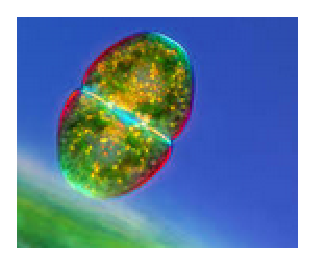
\includegraphics[width=0.3\textwidth]{fig1}
\end{minipage}
\hspace{0.05\linewidth}
\begin{minipage}{0.45\linewidth}
au revoir

\hyperlink{départ}{\beamerskipbutton{Départ}}

\href{run:geogebra.ggb}{\beamerskipbutton{Ficher Geogebra}}

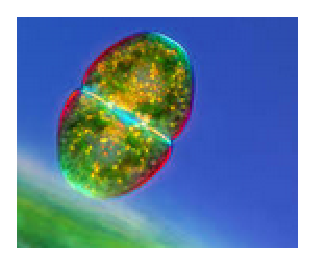
\includegraphics[width=0.3\textwidth]{fig1}
\end{minipage}
\end{frame}

%%%%%%%%%%%%%%%%%%%%%%%%%%%%%%%%%%%%%%%%%%%%%%%%%%%%%%%%%%%%

%\end{spacing}

%%%%%%%%%%%%%%%%%%%%%%%%%%%%%%%%%%%%%%%%%%%%%%%%%%%%%%%%%%%%
%%%%%%%%%%%%%%%%%%%%%
%% FIN DU DOCUMENT %%
%%%%%%%%%%%%%%%%%%%%%
\end{document}